\item As shown in the figure, in an experiment to determine Young’s modulus of a wire, the extension-load curve is plotted. The curve is a straight line passing through the origin and makes an angle of \(45^\circ\) with the load axis. The length of wire is 62.8cm and its diameter is 4mm. The Young’s modulus is found to be \(x \times 10^4 \text{Nm}^{-2}\). The value of \(x\) is \underline{\hspace{2.5cm}}.
    \begin{center}
        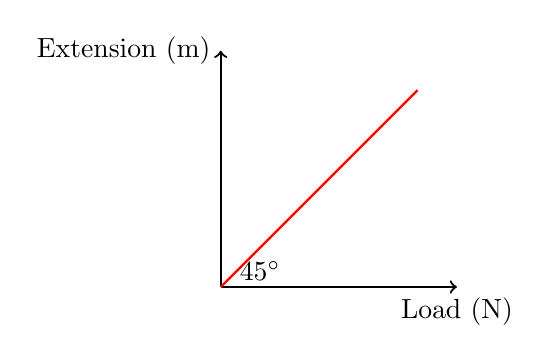
\begin{tikzpicture}
            \draw[->, thick] (0,0) -- (3,0) node[below] {Load (N)};
            \draw[->, thick] (0,0) -- (0,3) node[left] {Extension (m)};
            \draw[thick, red] (0,0) -- (2.5,2.5);
            \node at (0.5,0.2) {\(45^\circ\)};
        \end{tikzpicture}
    \end{center}